

\documentclass[]{emulateapj}
\usepackage{amsmath}

\usepackage[breaklinks,colorlinks,citecolor=blue,linkcolor=blue]{hyperref}
\usepackage{etoolbox}

\makeatletter

% Patch case where name and year are separated by aysep
\patchcmd{\NAT@citex}
  {\@citea\NAT@hyper@{%
     \NAT@nmfmt{\NAT@nm}%
     \hyper@natlinkbreak{\NAT@aysep\NAT@spacechar}{\@citeb\@extra@b@citeb}%
     \NAT@date}}
  {\@citea\NAT@nmfmt{\NAT@nm}%
   \NAT@aysep\NAT@spacechar\NAT@hyper@{\NAT@date}}{}{}

% Patch case where name and year are separated by opening bracket
\patchcmd{\NAT@citex}
  {\@citea\NAT@hyper@{%
     \NAT@nmfmt{\NAT@nm}%
     \hyper@natlinkbreak{\NAT@spacechar\NAT@@open\if*#1*\else#1\NAT@spacechar\fi}%
       {\@citeb\@extra@b@citeb}%
     \NAT@date}}
  {\@citea\NAT@nmfmt{\NAT@nm}%
   \NAT@spacechar\NAT@@open\if*#1*\else#1\NAT@spacechar\fi\NAT@hyper@{\NAT@date}}
  {}{}
  
\makeatother
%
\usepackage{xspace}
%
\usepackage{apjfonts}
\usepackage{amssymb, amsmath} % for e.g. \lesssim
\usepackage{natbibspacing, natbib}
\usepackage{aas_macros} % for understanding Journal in bib
\usepackage{graphics,graphicx}
%
\newcommand{\vdag}{(v)^\dagger}
\newcommand{\myemail}{tleung@astro.cornell.edu}
\newcommand{\Msun}{\mbox{$M_{\odot}$}\xspace}
\newcommand{\Rsun}{\mbox{$R_{\odot}$}\xspace}
\newcommand{\Lsun}{\mbox{$L_{\odot}$}\xspace}
\newcommand{\LIR}{\mbox{$L_{\rm IR}$}\xspace}
\newcommand{\LFIR}{\mbox{$L_{\rm FIR}$}\xspace}
%
\newcommand{\rarr}{$\rightarrow$}
\newcommand{\aco}{\mbox{CO($J$\,=\,1\,\rarr\,0) }}
\newcommand{\bco}{\mbox{CO($J$\,=\,2\,\rarr\,1) }}
\newcommand{\cco}{\mbox{CO($J$\,=\,3\,\rarr\,2) }}
\newcommand{\rot}[3][CO]{\mbox{#1($J$\,=\,#2\,\rarr\,#3)}}
%
\newcommand{\cii}{[C{\scriptsize II}]}
\newcommand{\Lp}[1][CO]{\mbox{$L^{\prime}_\textrm{\fontsize{8pt}{12pt}\selectfont{#1}}$}\xspace}
\newcommand{\kms}{\mbox{km\,s$^{-1}$}\xspace}
\newcommand{\LpU}{\mbox{K\,\,km\,\,s$^{-1}$\,\,pc$^2$}\xspace}
\newcommand{\pmOne}{\mbox{$^{-1}$}\xspace}
\newcommand{\alphaco}{\mbox{$\alpha_{\rm CO}$}\xspace}
\newcommand{\alphaU}{\mbox{$($K\,\,\kms\,\,pc$^2$$)$\pmOne}}
\newcommand{\sfrU}{\mbox{\Msun\,yr$^{-1}$}\xspace}
% Numerical values
\newcommand{\E}[1]{\mbox{$\times10^{#1}$}}
\newcommand{\petm}[2]{$^{+#1}_{-#2}$}
\newcommand{\eq}{\,=\,}
\newcommand{\pmm}{\,$\pm$\,}
%
\newcommand{\eg}{{e.g.,~}}
\newcommand{\ie}{{i.e.,~}}
%
\newcommand{\Fig}[1]{Figure~\ref{fig:#1}}
\newcommand{\Eq}[1]{Equation~\ref{eq:#1}}
\newcommand{\Tab}[1]{Table~\ref{tab:#1}}
\newcommand{\Sec}[1]{\S\ref{sec:#1}}
%
\newcommand\tna{\,\tablenotemark{a}}
\newcommand\tnb{\,\tablenotemark{b}}
\newcommand\tnc{\,\tablenotemark{c}}
\newcommand\tnd{\,\tablenotemark{d}}
\newcommand\tne{\,\tablenotemark{e}}
\newcommand\tnf{\,\tablenotemark{f}}
\newcommand\tng{\,\tablenotemark{g}}
\newcommand\tnh{\,\tablenotemark{h}}
\newcommand\tni{\,\tablenotemark{i}}
\newcommand\tnj{\,\tablenotemark{j}}
\newcommand\tnk{\,\tablenotemark{k}}
\newcommand\tnl{\,\tablenotemark{l}}
%
\def\herschel {{\it Herschel Space Observatory}\xspace}
\def\alma     {Atacama Large (sub-)Millimeter Array (ALMA)\xspace}
\def\spitzer {{\it Spitzer Space Telescope}\xspace}
\def\pdbi     {Plateau de Bure Interferometer\xspace}
\def\carma    {Combined Array for Research in Millimeter-wave Astronomy\xspace}
\def\cso      {Caltech Sumillimeter Observatory (CSO)\xspace}
\def\noema    {Northern Extended Millimeter Array (NOEMA)\xspace}
\def\vla      {{\it Karl G. Jansky} Very Large Array\xspace}
% Typography
\newcommand{\ncode}[1]{{\sc #1}}
% Codes / Softwares
\newcommand{\uvmcmcfit}{\ncode{uvmcmcfit}\xspace}
\def\aips {\ncode{AIPS}\xspace}
\def\casa {\ncode{CASA}\xspace}
% Long words
\newcommand{\lowZ}{low-metallicity\xspace}
\newcommand{\mulw}{multi-wavelength\xspace}
\newcommand{\SF}{star formation\xspace}
\newcommand{\SB}{starburst\xspace}
\newcommand{\SBs}{starbursts\xspace}
\newcommand{\gl}{gravitationally lensed\xspace}
\newcommand{\MCMC}{Markov Chain Monte Carlo (MCMC)\xspace}
% Wavelength regimes
\newcommand{\fir}{far-IR\xspace}
\newcommand{\fuv}{far-UV\xspace}
\newcommand{\mir}{mid-IR\xspace}
\newcommand{\nir}{near-IR\xspace}
\slugcomment{To be submitted to the ApJ}

\citestyle{aa}
\shorttitle{TBD}
\shortauthors{Leung \& Riechers}

\begin{document}
%{\tiny  \RevisionInfo}

\title{Gas Dynamics of the Einstein ring RXSJ1131-1123 at $z$=0.654}
\author{T. K. Daisy Leung and Dominik A. Riechers}
\affil{Department of Astronomy, Space Sciences Building, Cornell University,
Ithaca, NY 14853, USA; \myemail}


\begin{abstract}
\end{abstract}

\section{Introduction} 
The gravitational lens RXJ 1131-1231 was discovered with spectroscopic
redshifts of the lens and the QSO are $z_{\rm L}$ = 0.295 and
$z_\textrm{AGN,HST}$ = 
0.658, respectively \citep{}

% FG gal is an elliptical gal: Slues+03 absorption lines  


As detected in the HST images, RXJ1131-1231 is a quadruply imaged AGN with
Einstein ring of size 1\farcs83 in radius. The 
background AGN is lensed into 4 point-like image A,B,C,D on a ring (emission
from the AGN host galaxy) around G, the foreground galaxy. 
C06 report the redshift of the background AGN of 0.658 with magnification ~ 9,
claimed Seyfert 1 spiral galaxy.




\section{Observations}
\subsection{PdBI} \label{sec:PdBIdata}
Observations of the CO($J$ = 2 $\rightarrow$ 1) rotational line ($\nu_{\rm
rest}$ = 230.5379938 GHz) toward the background galaxy RXJ1131-1231 at $z$ =
0.654
 were carried out using IRAM Plateau de Bure Interferometer (PdBI) at the
(Program ID: S14BX001; PI: D. Riechers). 
 Two observing runs were carried out on 2014 Dec 06 and 2015 Feb 05 under good
weather conditions in the C and D array configurations, respectively. The 2 mm
receivers were used to cover the redshifted CO($J$ = 2 $\rightarrow$ 1) line
and the 
underlying continuum emission (rest-frame 3.6 mm), employing
a correlator setup providing an effective bandwidth of 3.6 GHz and spectral 
resolution of 10.0 MHz ($\sim$21.5281 km s$^{-1}$).
This resulted in 3.74 hours of cumulative six antenna-equivalent on-source time
after discarding unusable visibility data.
% D: 1.5 hours; 1055+018 (BP) , 3C279 (RF, fixed flux), 1127-145 (phase/amp),
% 1124-186(ditto)
% C: 2.2 hours; MWC349 (fixed flux), 1055+018 (RF = bandpass), 1124-186
% (phase/amp), 1127-145 (ditto)
% total: 3.75 hours
%For both tracks, 
The nearby quasars 1127$-$145 and 1124$-$186 were observed every 22 minutes
for
pointing, secondary amplitude, and phase calibration and 1055$+$018 was
observed as bandpass calibrators 
for both tracks.
MWC349 and 3C279 were observed
as the primary
absolute flux calibrator for C and D array observations, respectively, yielding
$\lesssim
$15\% calibration accuracy.

The GILDAS package was used to reduce and analyze the visibility data which are
then imaged and deconvolved using
the CLEAN algorithm with ``natural" weighting. This yields a synthesized clean
beam size of 4$\farcs$44 $\times$ 1\farcs95 (PA: 13\degr). The final rms noise
is $\sigma$ =
0.177 
Jy km s$^{-1}$ beam$^{-1}$ over a channel width of 320 MHz (corresponding to
690 km s$^{-1}$), and $\sigma$ = 1.451 Jy km s$^{-1}$ beam$^{-1}$ over 10 MHz 
(21.5 km s$^{-1}$) . 
The continuum image is created by % 2.152 mm; 
averaging over all the line-free channels ($\nu_{\rm cont}\sim$139 GHz). This
yields an rms noise of 0.082 mJy beam$^{-1}$. % see README.md in 04Sep15

\subsection{CARMA} \label{sec:carmadata}
% LO = 215.6694 Ghz
% 1127-189 Gain for set 2
% 3C273 gain for set 3
% 3C279 Bandpass for both
% mars flux for both
% after flagging: Total observing time is  1.48 hours, checked with uvindex for
% set 3
% after flagging: Total obs. time is 2.94 hours, checked with uvindex for the
% combined set
% 12.500 GHz <=> 17.935 km/s
%
Observations of the CO($J$ = 3 $\rightarrow$ 2) rotational line ($\nu_{\rm
rest}$ = 345.7959899 GHz) 
%toward the background galaxy RXJ1131-1231 at $z$ = 0.654
 were carried out using the Combined Array for Research in Millimeter-wave
Astronomy (CARMA; Program ID: cf0098; PI: D. Riechers) on 2014 February 17 
under good 3 mm weather
conditions and on 2014 February 02 under terrible 3mm weather in the D array
configurations.  The 3 mm receivers were used to cover
the 
redshifted CO($J$ = 3 $\rightarrow$ 2) line, employing a correlator setup
providing a bandwidth of 3.75 GHz in each sideband and spectral resolution of
12.5 MHz ($
\sim$17.9 km s$^{-1}$). The line was placed in the
lower sidebands with the local oscillator tuned to $\nu_{\rm LO}\sim$ 216 GHz;
this resulted in 2.94 hours of 15 antenna-equivalent on-source time after
flagging poor visibility data. 
The radio quasars 3C273 and J1127-189 was observed every 15 minutes for
pointing, amplitude, and phase calibration. Mars was observed as the
primary
absolute flux calibrator and 3C279 was observed as bandpass calibrators for
both tracks. 
% poor phase note
Since the phase calibrator from the first track is faint and was observed under
poor weather and the phase calibrator used for the second track was
far from our target source.
Hence, the phase calibration was 
subpar, with rms scatter $\sim$ 60\degr. 
We estimate $\sim
$BLAH\% calibration accuracy based on the flux scale uncertainties, gain variation over time, and 
the calibrated phase scatter.
The MIRIAD package was used to calibrate and analyze the visibility data which
are imaged and deconvolved using
the CLEAN algorithm with ``natural" weighting. This yields a synthesized clean
beam size of 3\farcs2 $\times$ 1\farcs9 (PA: 8\degr) for the lower sideband
image cube. The
final 
rms noise is $\sigma$ = 13.3 mJy km s$^{-1}$ beam$^{-1}$ over a channel width
of
25 MHz (corresponding to 35.87 km s$^{-1}$). 

\subsection{VLA} 
% 20081229
% flux 1331+305
% phase 1130-149

Observations of the radio continuum toward the
galaxy RXJ1131-1231 were carried out using the {\it Karl G. Jansky} Very Large 
Array (VLA; Program ID: AW741; PI: Wucknitz).
Observations were carried out on BLAH under excellent/GOOD? weather
conditions in the A array configurations. The C-Band receivers were used to 
cover the BLAH
, employing a correlator setup providing a bandwidth of BLAH GHz in each
sideband. This resulted in BLAH hours of BLAH antenna-equivalent on-source time
after 
discarding unusable visibility data.

The nearby radio quasar BLAH was observed every BLAH minutes for
pointing, amplitude, and phase calibration, and BLAH was observed as the
primary
absolute flux calibrator. BLAH were observed as bandpass calibrators, yielding
$\sim
$15\% calibration accuracy.
The AIPS package was used to calibrate and analyze the visibility data which
are imaged and deconvolved using
the CLEAN algorithm with ``natural" weighting. This yields a synthesized clean
beam size of 2$\farcs$6 $\times$ 2\farcs2 for the continuum image. The final
rms 
noise is $\sigma$ = 0.68 Jy km s$^{-1}$ beam$^{-1}$.




\section{\rot{2}{1} Lens model}

\subsection{interpretation}
- C06 suggest the presence of an interacting dusty galaxy in their HST
observations, which BJB+08 calls it the F component. The lensed images of the
ABCDE 
components coincide with our CO data (see mom0 on HST and channel map),
evidently CO emission coming from the AGN host galaxy. 
- one of the red channels in our lens model suggests a second source component,
which is consistent with the spatially offset dusty source (see mom0 on HST,
which 
the red velocity component coincides with this F component)

%%%%%%%%%%%%%%%%%%%%%%%%
We compare our lens model parameters on the mass distribution of the lensing
galaxy with literature, particularly against the SIE model presented by C06. 
In C06, their SIE model shows position of lensing mass is offset by (-0.015",
-0.041" from obsservations (i.e. light centroid)); PA = -73.6, ellipticity = 0.45,
theta\_R = 1.84" $\pm$ 0.01. 
Our best-fit model parameters finds a BLAH
	- Our model lens parameters (median):
		- file: WRITEUP/MedianLensModelParams.txt
		- lensing gal. position is consistent with C06, 
		- Einstein radius: consistent with C06
		- PA: consistent within errors
		- Axial ratio: consistent within errors
%%%%%%%%%%%%%%%%%%%%%%%%%

Differential lensing is at play as suggested by the spectral shape of the \rot{2}{1} line profile, where 
flux density in the red wing is much high than in the blue wing.  
We modelled the emission using different kinematic components, the magnification factors are reported in Table BLAH.
\begin{deluxetable}{lcc}[!htbp]
\tabletypesize{\scriptsize}
\tablecolumns{3}
\tablecaption{Magnification factors of various kinematic components in \bco}
\tablehead{
\colhead{Velocity Range(\kms)} & % see 22May16/intensity30Apr16.spec; or channel map in paper
\colhead{Source 1 $\mu_{\rm L}$} &
\colhead{Source 2 $\mu_{\rm L}$}
}
\startdata
$-$366\,$-$\,$-$258 & 3.1 $\pm$ 0.9 & \\ [0.5ex]
$-$237\,$-$\,$-$151 & 4.3 $\pm$ 2.4 & \\ [0.5ex]
$-$129\,$-$\,$-$43  & 4.2 $\pm$ 0.6 & \\ [0.5ex]
$-$21.5\,$-$\,65    & 4.1 $\pm$ 0.9 & \\ [0.5ex]
86\,$-$\,172        & 8.7 $\pm$ 2.0 & \\ [0.5ex]
194\,$-$\,280       & 7.6 $\pm$ 1.6 & \\ [0.5ex]
301\,$-$\,388       & 7.2 $\pm$ 5.6 & 6.7 $\pm$ 2.5 \\ [0.5ex]
weighted average & 4.4 & \\ [0.5ex]
median & 5.5 &
\enddata
\label{tab:model}
\tablecomments{Velocity is taken from the center of each (native) channel
without any binning. Each row corresponds to a channel slice used for
lens modeling. Source 1 is RXJ1131 and source 2 is its companion. See text for details. }
\end{deluxetable}


\begin{figure}[tbph]
\centering
\includegraphics[width=0.50\textwidth]{../Figures/Pseudointegrated_datamodel.eps}
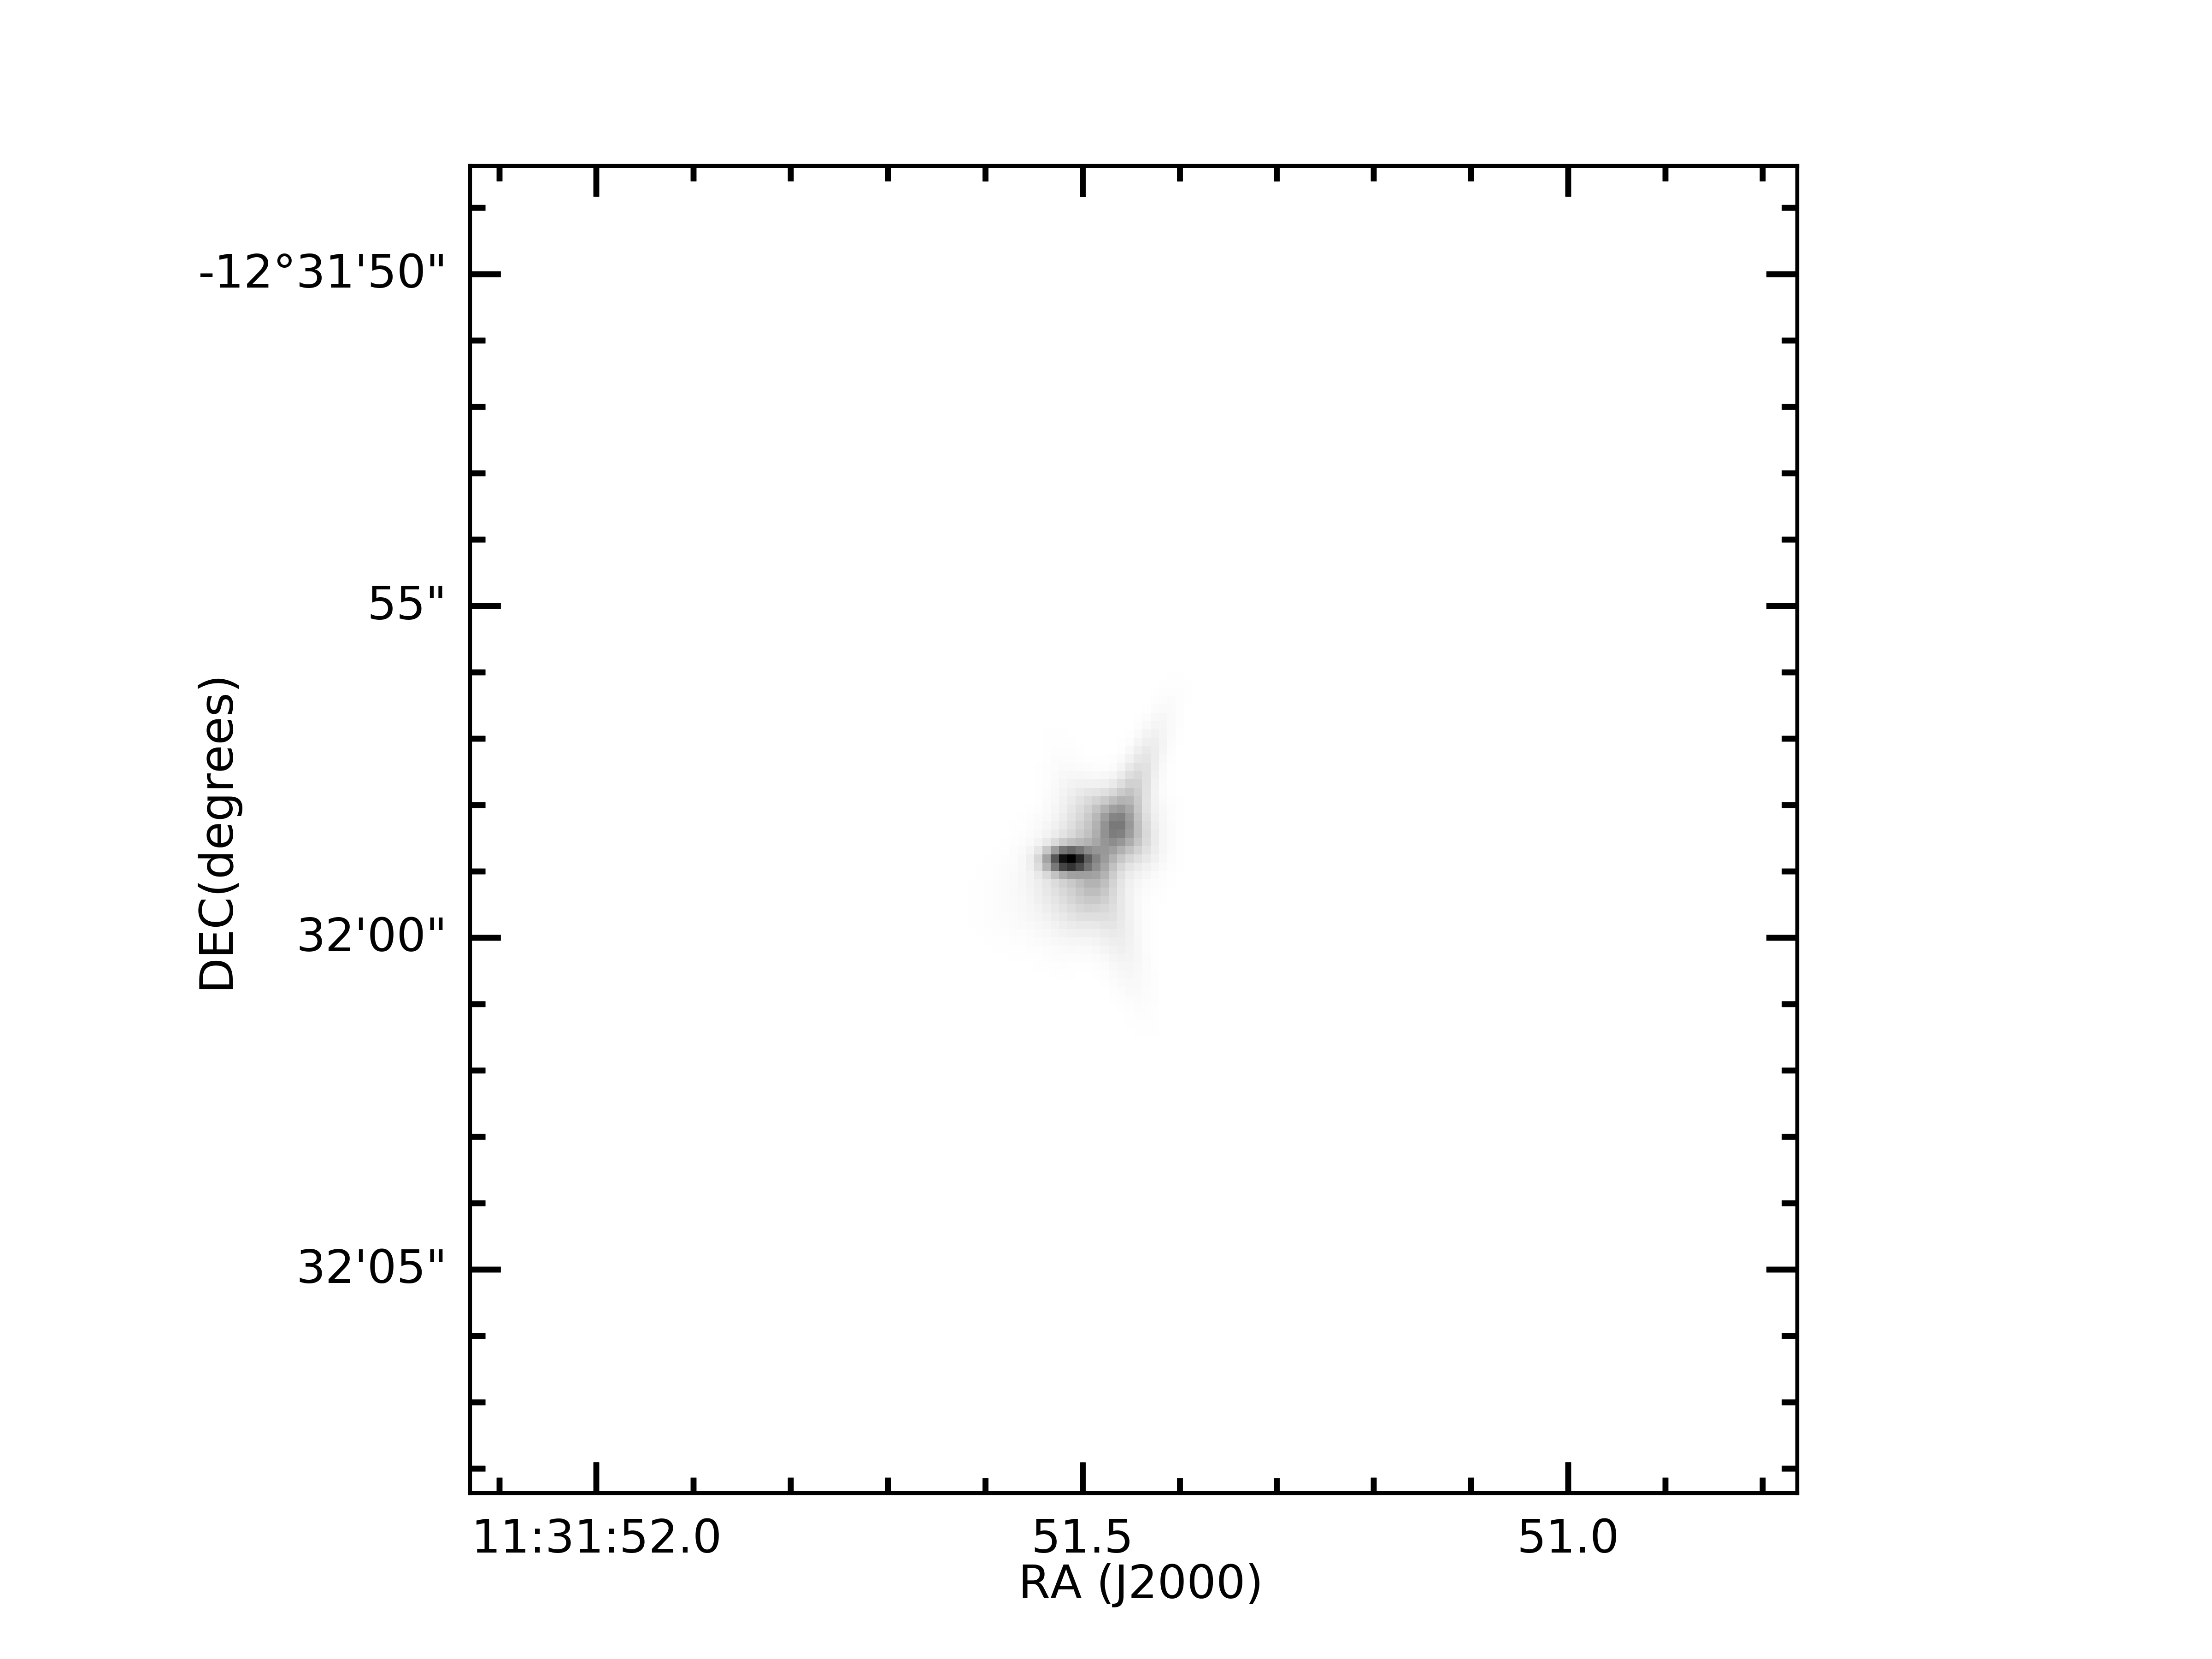
\includegraphics[width=0.50\textwidth]{../Figures/SourcesPlane.png}
\caption{
Pseudo observed 0th moment map in the lens plane. (left)
Pseudo 0th moment map in the source plane. (right)
\label{fig:}}
\end{figure}


\begin{figure*}[tbph]
\centering
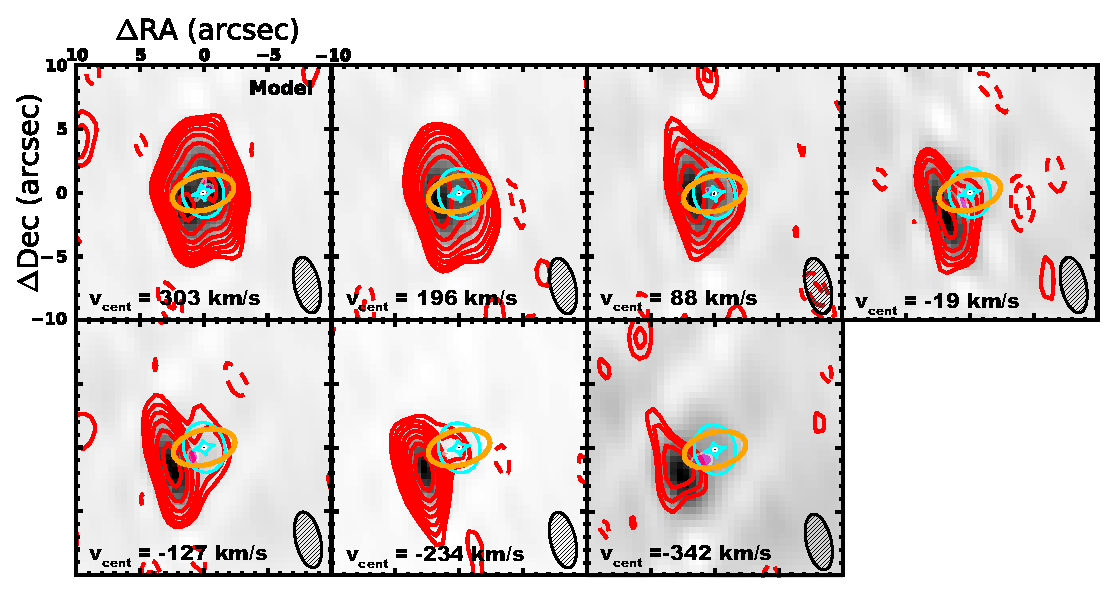
\includegraphics[width=0.65\textwidth]{../Figures/PostageStampModel.eps}
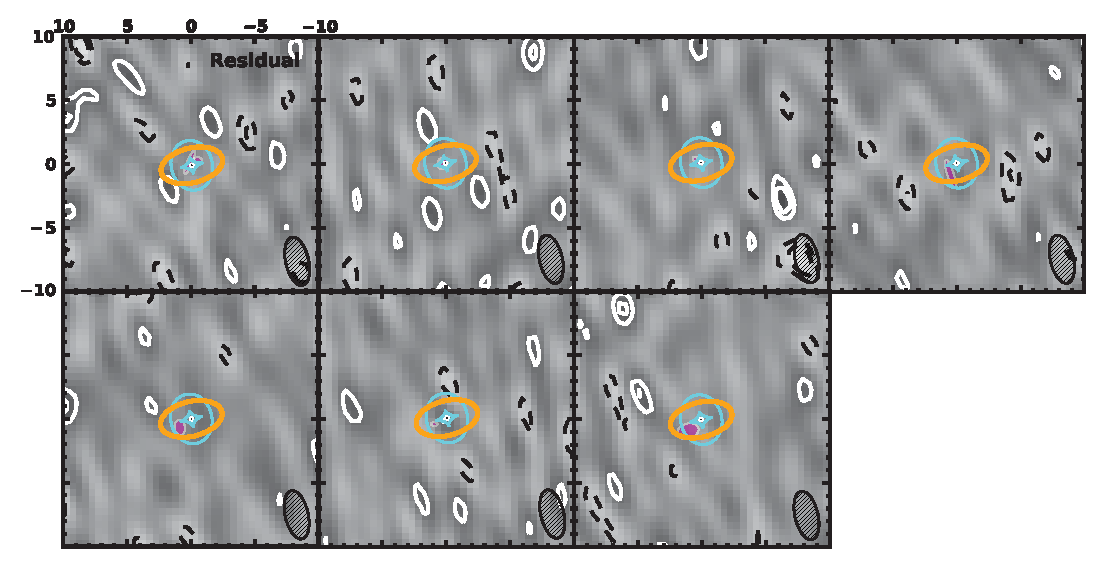
\includegraphics[width=0.65\textwidth]{../Figures/PostageStampResiduals.eps}
\caption{
of channel widths $\sim$ 100\kms. 
\label{fig:}}
\end{figure*}


\begin{figure}[tbph]
\centering
\includegraphics[width=0.80\textwidth]{../Figures/PseudoRGB_Lensed_SB_double.eps}
\caption{
velocity gradient of the lens model in the lens plane (left), source plane
(right).
\label{fig:}}
\end{figure}


%\begin{figure*}[tbph]
%\centering
%\includegraphics[width=0.8\textwidth]{}
%\includegraphics[width=0.65\textwidth]{}
%\caption{
%\label{fig:}}
%\end{figure*}
\end{document}